\begin{figure}
    \centering
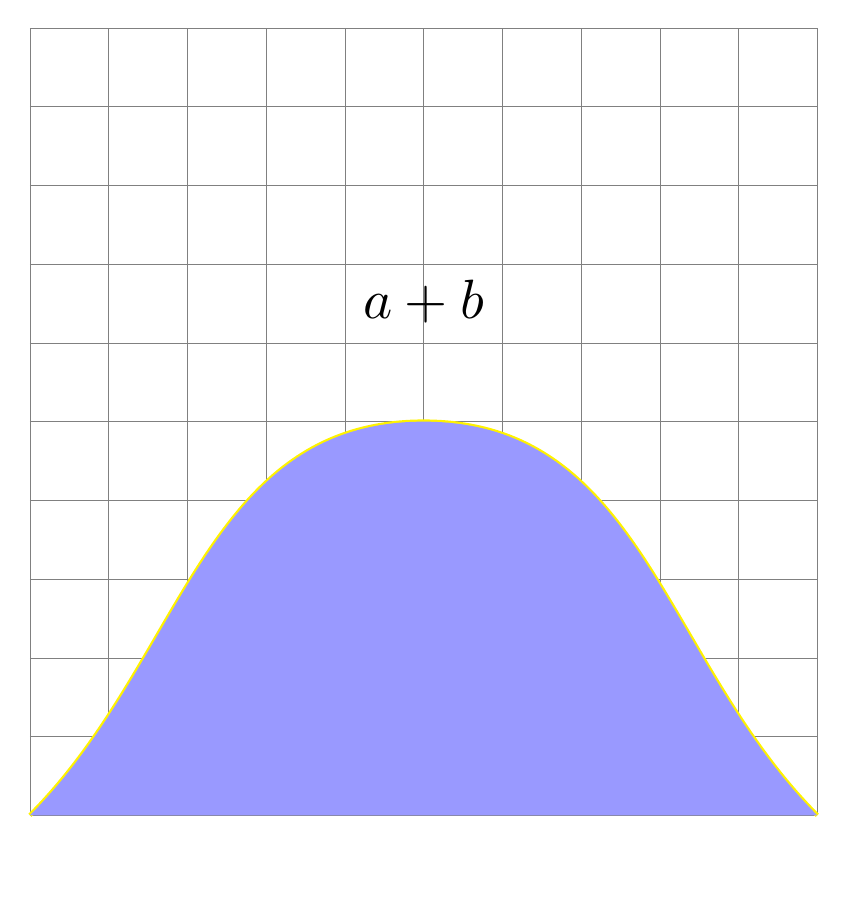
\begin{tikzpicture}[scale = 1]
    \draw [scale = 1,help lines] (0,0) grid (10,10);
    
    %\draw[ultra thick,scale = 3,<->] (0,0) -- (3,3);
    
    %\draw[line width = 1 pt,<->](0,10) -- (0,-5);
    
    %\draw[green,line width = 3pt,<->,rounded corners](0,5) -- (5,0);
    
    %\draw[red,line width = 3pt,->,rounded corners](1,0) -- (4,0) -- (4,4) -- (1,4);
    
    \draw[red,ultra thick, domain = 5:5,samples = 10] plot (\x,{sin(\x r)});
    
    \draw[yellow,ultra thick] (0,0) to [in = 180 ,out =45] (5,5) to [in = 135 ,out = 0](10,0);
    \path[fill = blue!40!white] (0,0) to [in = 180 ,out =45] (5,5) to [in = 135 ,out = 0](10,0);
    
    \node[scale = 2,anchor = south] at (5,6) {$a + b$};
\end{tikzpicture}    
    \caption{Caption}
    \label{fig:my_label}
\end{figure}